%-----------------------------------------------------------------------------
%
%               Template for sigplanconf LaTeX Class
%
% Name:         sigplanconf-template.tex
%
% Purpose:      A template for sigplanconf.cls, which is a LaTeX 2e class
%               file for SIGPLAN conference proceedings.
%
% Author:       Paul C. Anagnostopoulos
%               Windfall Software
%               978 371-2316
%               paul@windfall.com
%
% Created:      15 February 2005
%
%-----------------------------------------------------------------------------


\documentclass[preprint]{sigplanconf}


% The following \documentclass options may be useful:
%
% 10pt          To set in 10-point type instead of 9-point.
% 11pt          To set in 11-point type instead of 9-point.
% authoryear    To obtain author/year citation style instead of numeric.

\usepackage{amsmath}
\usepackage{amssymb}
\usepackage{listings}
\usepackage[pdftex]{graphicx}
\usepackage{epsfig}
\usepackage{verbatim} % only for comment environment
\usepackage{ifthen}
\usepackage{needspace}
\usepackage{url}

\urlstyle{sf}

\graphicspath{{figures/}}
\DeclareGraphicsExtensions{.pdf, .png, .ps}   % NOT .jpg  because it throws away the detail.

\newboolean{showcomments}
\setboolean{showcomments}{true}
\ifthenelse{\boolean{showcomments}}
  {\newcommand{\nb}[2]{
    \fbox{\bfseries\sffamily\scriptsize#1}
    {\sf\small$\blacktriangleright$\textit{#2}$\blacktriangleleft$}
    % \marginpar{\fbox{\bfseries\sffamily#1}}
   }
  }
  {\newcommand{\nb}[2]{}
  }
\newcommand\apb[1]{\nb{apb}{#1}}
\newcommand\spj[1]{\nb{spj}{#1}}
\newcommand\je[1]{\nb{jeff}{#1}}

\begin{document}

\lstset{language=Haskell, basicstyle=\footnotesize, numbers=none, numberstyle=\footnotesize, stepnumber=1, numbersep=5pt, showspaces=false, showtabs=false, frame=none, tabsize=2, captionpos=b, breaklines=true, breakatwhitespace=false, xleftmargin=10pt,showstringspaces=false}
% ,resetmargins=true,breakindent=1cm,breakautoindent=true

% from http://www.haskell.org/haskellwiki/Literate_programming
\lstnewenvironment{code}
    {\lstset{}%
      \csname lst@SetFirstLabel\endcsname}
    {\csname lst@SaveFirstLabel\endcsname}
    \lstset{
      basicstyle=\small\sffamily,
      flexiblecolumns=false,
      basewidth={0.5em,0.45em},
      literate={+}{{$+$}}1 {/}{{$/$}}1 {*}{{$*$}}1 {=}{{$=$}}1
               {>}{{$>$}}1 {<}{{$<$}}1 {\\}{{$\lambda$}}1
               {\\\\}{{\char`\\\char`\\}}1
               {->}{{$\rightarrow$}}2 {>=}{{$\geq$}}2 {<-}{{$\leftarrow$}}2
               {/=}{{$\neq$}}1
               {<=}{{$\leq$}}2 {=>}{{$\Rightarrow$}}2 
%               {\ .}{{$\circ$}}2 {\ .\ }{{$\circ$}}2
               {...}{{\textrm{ \ldots}}}1
               {>>}{{$\gg$}}2 {>>=}{{$\gg=$}}2
               {|}{{$\mid$}}1               
    }


\conferenceinfo{ICFP 2011}{date, City.} 
\copyrightyear{2011} 
\copyrightdata{[to be supplied]} 

\titlebanner{Haskell for the cloud}        % These are ignored unless
\preprintfooter{Haskell for the cloud}   % 'preprint' option specified.

%\renewcommand{\textfraction}{0.05}
%\renewcommand{\topfraction}{0.9}
%\renewcommand{\bottomfraction}{0.8}
%\renewcommand{\floatpagefraction}{0.7}
%\setcounter{totalnumber}{5}


%%%%% Andrew's commands
\newcommand{\ct}[1]{\textsf{#1}}

\newcommand{\nfn}{\ensuremath{\stackrel{\hash}{\rightarrow}}}
\newcommand{\nlambda}{\ensuremath{\lambda^\hash}\,}
\newcommand{\napp}{\ensuremath{\;\ct{\small \$}^{\hash}\,}}

\newcommand{\Int}{\mathbb{Z}}
\newcommand{\pair}[2]{\mbox{$\langle$#1, #2$\rangle$}}
\newcommand{\mpair}[2]{\mbox{$\langle #1, #2 \rangle$}}
\newcommand{\entails}{\vdash}
\newcommand{\hash}{\texttt{\#}}
\newcommand{\closed}[1]{\hash\,#1}
\newcommand{\textt}[1]{\lstinline!#1!}
\newcommand{\kmeans}{$k$-means}





\title{Haskell for the cloud}
\subtitle{}

\authorinfo{Jeff Epstein}
           {University of Cambridge}
           {jee36@cam.ac.uk}
\authorinfo{Andrew P. Black}
           {Portland State University\titlenote{Research conducted while on sabbatical at Microsoft Research, Cambridge.}}
           {black@cs.pdx.edu}
\authorinfo{Simon Peyton-Jones}
           {Microsoft Research, Cambridge}
           {simonpj@microsoft.com}

\maketitle
\begin{abstract}
% 1. What's the problem?
% 2. What does it matter?
% 3. What's the solution?
% 4. What are the consequences?
We present Cloud Haskell, a domain-specific language for developing programs for a distributed-memory computing environment. Implemented as a shallow embedding in Haskell, it provides a message-passing communication model, inspired by Erlang, while retaining compatibility with Haskell's established shared-memory concurrency. We believe that Cloud Haskell will let programmers create fault-tolerant, high-performance distributed systems with a minimum of effort, while retaining Haskell's strengths in strong typing and shared-memory concurrency.

\end{abstract}


%\category{D.1.3}{Programming Techniques}{Concurrent Programming---Distributed Programming}
%\category{D.3.2}{Programming Languages}{Haskell}
%
%
%\terms
%Languages, Reliability, Performance, Distribution
%
%\keywords
%Haskell, Erlang, message-passing
%
\section{Introduction}

With the age of steadily-improving processor performance behind us, we must learn to compute with more, rather than faster, processors. 
A \emph{cloud} is data center that makes available a large number of processors for storing and processing users' data; we'll use this term to mean specifically a network of computers that have independent failure modes and separate memories.

How should we program the cloud?  One approach is to simulate a familiar shared-memory multiprocessor, and then to program the simulated computer using shared-memory concurrency primitives, such as locks and transactions. 
%We have two objections to this approach.  The first is that the preponderance of the evidence is that shared-memory concurrency is \emph{just too hard}.  
%\spj{Not a strong argument.  Message passing is always available for shared memory machines and people don't use it much.  It's just
%too inconvenient, or its cost model doesn't fit.  I'd nuke this objection.}
%For example, 
%$<<$Automatically classifying benign and harmful data races using replay analysis?$>>$
Although possible, we don't believe this to be the best way forward.
To be effective, a programming model must be accompanied by a cost model: it must give programmers tools for reasoning about the cost of computation.  In a distributed memory system, one of the most significant costs, in both energy and time, is data movement.
A programmer trying to reduce these costs needs a model in which they are explicit, not one that denies that data movement is even taking place\,---\,which is exactly the premise of a simulated shared memory. 
Synchronization is another major cost; while shared memory makes some synchronization explicit (locks, compare and swap), the synchronization implicit in the simulation of the memory itself, and in higher-level abstractions such as transactions, remains implicit.

Instead, we turn to a solution popularized by \mbox{Erlang}\,\cite{Erlang93} and MPI\,\cite{mpi99}: {\em message passing}. The message-passing model stipulates that the concurrent processes have no access to each other's data: any data that needs to be communicated from one process to another are explicitly sent in {\em messages}.  This make the costs of communication apparent.
It also means that a concurrent process is natural unit of failure: since processes do not share data, the data of one process cannot be contaminated by a fault in another.
%Of course, it is possible that a failing process sends a corrupted or misleading message, but this is a much narrower channel than the ability to write willy-nilly into memory.

Failure is, in many ways, \emph{the} defining issue of distributed computation.  In a network of hundreds of computers, some of them are likely to fail during the course of an extended computation; if our only recourse were to restart the computation from the beginning, the likelihood of it ever completing would become ever smaller as the system scales up.  
A programming system for the cloud must therefore be able to tolerate partial failure.  Here again, Erlang has a solution that has stood the test of time; 
%the highest reliability programs on the planet are written in Erlang, and achieve 9 nines reliability.  We 
we don't innovate in this area, but adopt Erlang's solution (summarized in Section \ref{FaultTolerance}).

Cloud Haskell is a domain-specific language for cloud computing, implemented as a shallow embedding in Haskell.
It presents the programmer with a computational model  similar to Erlang's, but with additional advantages that stem from Haskell's purity, types, and monads.  
As a pure functional language, data is by default immutable, so shared, mutable data won't be missed.  
More importantly, the implementation can decide whether to share or copy immutable data: the choice is semantically invisible. 
Moreover, pure functions are idempotent; this means that functions running on failing hardware can be restarted elsewhere without the need for distributed transactions or other mechanisms for ``undoing'' effects.  
Types in general, and monadic types in particular, help to guarantee properties of programs statically.  
For example, a function that has an externally-visible effect such as sending or receiving a message \emph{cannot} have the same type as one that is pure.
Monadic types make it convenient to program in an effectful style when that is appropriate, while ensuring that the programmer cannot accidentally mix up the pure and effectful code.

The contributions of this paper are:
\vspace{-1ex}
\begin{itemize}
\item A description of Cloud Haskell's interface functions. (Section \ref{s:processes}). Following the Erlang model, our language provides a system for exchanging messages between concurrent processes, regardless of whether those threads are running on one computer or on many. We also provide functions for starting new remote processes, and for fault tolerance, which closely follow Erlang. 
However, unlike Erlang, Cloud Haskell supports allows shared-memory concurrency \emph{within} one of its concurrent processes.

\item A method for serializing function closures to enable higher-order functions to work in a distributed environment (Section \ref{s:closures}). Starting a remote process means sending a representation of a function and its environment across the network;  our approach makes the environment \emph{explicit}, and thus gives the programmer control over the cost of the message.

\item A demonstration of the effectiveness of our approach in the form of an example application and performance measurements from the $k$-means clustering algorithm, an iterative algorithm for partitioning data points into natural groups (Sections \ref{s:completeApp} and \ref{s:performance}). The highly parallel nature of this algorithm makes it well-suited for deployment in a distributed environment.
\end{itemize}
\pagebreak

\section{Processes and messages}
We start with an overview of the basic elements of Cloud Haskell:
processes, messages, what can be sent in a message and provision for failure.
All of the elements of our DSL are listed in Figure~\ref{fig:api}.
\subsection{Processes}
%: \label{s:Processes}
\label{s:processes}
The basic unit of concurrency in Cloud Haskell is the {\em process}:  a concurrent activity that has been ``blessed'' with the ability to send and receive messages. As in Erlang, processes are lightweight, with low creation and scheduling overhead.  Processes are identified by a unique process identifier, which can be used to send messages to the new process.

In most respects, Cloud Haskell follows Erlang by favoring message-passing as the primary means of communication between processes. Our language differs from Erlang, though, in that it also supports shared-memory concurrency within a single process. The existing elements of Concurrent Haskell, such as \textt{MVar} for shared mutable variables and \textt{forkIO} for creating lightweight threads, are still available to programmers who wish to combine message passing with the more traditional approach. This is illustrated in Figure~\ref{fig:ProcessBubbles}. Our embedding ensures that mechanisms specific to shared-memory concurrency cannot be inadvertently used between remote systems.  The key idea that make this separation possible is that not all data types can be sent in a message; in particular, \textt{MVar}s and \textt{ThreadId}s are not Serializable.
We discuss this point further in Section~\ref{s:serialization}.

\begin{figure}[t]
\centerline {
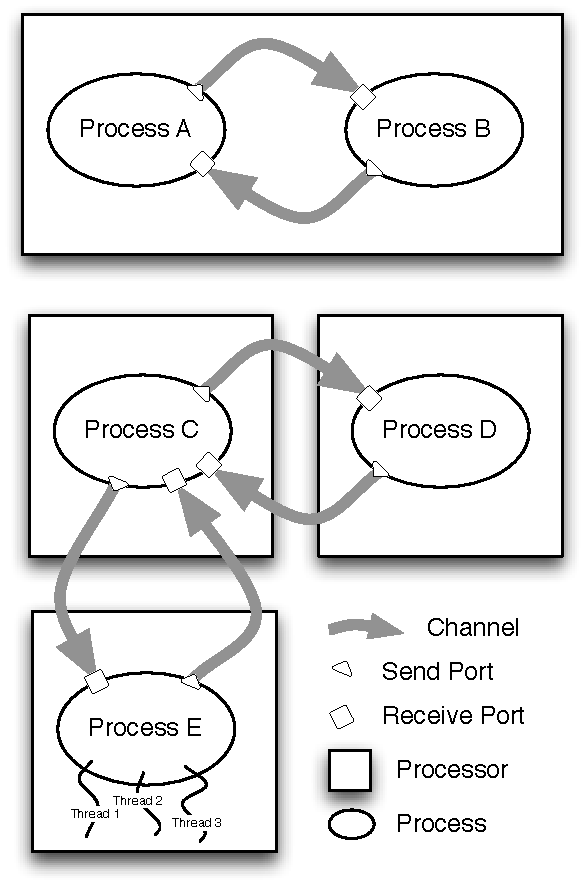
\includegraphics[width=\columnwidth]{threadsAndProcesses}
}
\caption{ 
%: \label{fig:ProcessBubbles}
\label{fig:ProcessBubbles}
Processes A and B do not share memory, even though they are running on the same physical processor, that is, the same node. Instead they communicate by sending messages, shown by grey arrows.  This makes it easy to reconfigure the application to resemble the situation shown with processes C and D.  Process E has created some lightweight threads using Concurrent Haskell's \texttt{forkIO} primitive; these threads share memory with Process E and with each other.  However, they cannot send or receive messages from Process E's channels, because this requires execution in the \texttt{ProcessM} monad; threads, in contrast, execute in the \texttt{IO} monad.
}
\end{figure}


\subsection{Messages to processes}
%: \label{s:sendAndExpect}
\label{s:sendAndExpect}

Any process can send and receive messages. Our messages are asynchronous, reliable, and buffered.  All the state associated with messaging (most especially, the message queue) is wrapped in the \textt{ProcessM} monad, which is updated with each messaging action. Thus, any code participating in messaging must be in the \textt{ProcessM} monad.  The basic primitives are \textt{send} and \textt{expect}\footnote{Why \textt{expect} rather than \textt{receive}?  The intent is that \textt{expect} is used when the program \emph{expects} a message of a particular type.  
There are more general \textt{receive} functions that allow for type-dependent and conditional receives;  these are discussed in Section~\ref{s:matching}.}:

\par{\small
\begin{code}
send :: (Serializable a) => ProcessId -> a 
						-> ProcessM ()
expect :: (Serializable a) => ProcessM a
\end{code}}
\noindent

Before we discuss these primitives in detail, let's look at an example of their use.
\textt{ping} is a process that accepts ``pong'' messages and responds by sending a ``ping'' to whatever process sent the pong. Using \textt{send} and \textt{expect}, the code for such a process would look like this:

\begin{code}
data Ping = Ping ProcessId
data Pong = Pong ProcessId
-- omitted: Serializable instance for Ping and Pong

ping :: ProcessM ()
ping = do { self <- getSelfPid
          ; Pong partner <- expect
          ; send partner (Ping self)
          ; ping }
\end{code}

\noindent The equivalent code in Erlang looks like this:

\begin{lstlisting}[language=Erlang]
ping() -> receive
           {pong, Partner} -> 
              Partner ! {ping, self()}
          end,
          ping().               
\end{lstlisting}

These two programs have similar structure. Both \textt{ping} functions are designed to be run as processes. They each wait for a specific message to be received; the Haskell \textt{expect} function matches incoming messages by type, whereas in Erlang, messages are usually pattern-matched against tuples whose first element is a well-known atom. The programs wait for a ``pong'' message, and ignore all others. The ``pong'' message contains in its payload the process ID of a ``partner'', to whom the response message is sent; this message contains the process ID of the \textt{ping} process (\textt{self}). Finally, they wait for the next message by repeating with tail recursion.

%If this example looks familiar, it should: it's very close to the first distributed programming example given in {\em Getting Started with Erlang}\cite{GSWE}. 
Note that in the Erlang version, \textt{Ping} and \textt{Pong} are atoms, whereas in the Haskell version they are types, and so need to be declared explicitly. 
As given, the type declarations are incomplete; \textt{Ping} and \textt{Pong} need to be declared to be instances of the class \textt{Serializable}; we will discuss this in Section~\ref{s:serialization}.

The \textt{send} function is our general-purpose message-sending primitive; it packages up a chunk of \emph{serializable} data of arbitrary type as a bag of bits, 
together with a representation of that type (a \textt{TypeRep}), and transmits both (possibly over the network) to a particular process, selected by the \textt{ProcessId} argument.
Upon receipt, the incoming message will be placed in a message queue associated with the destination process. 
The \textt{send} function corresponds to Erlang's \textt{!} operator.

At the far end of the channel, the simplest way of receiving a message is with \textt{expect}, which
examines the message queue associated with the current process and extracts the first message whose type matches the (inferred) type of \textt{expect}\,---\,a \textt{Ping} message in the example.  
The implementation of \textt{expect} looks down the queue for a message with the right type representation, 
dequeues that message, parses the bag of bits into a data item of the right type, and returns it.
If there is no message of the appropriate type on the queue, \textt{expect} waits for one to arrive.

\subsection{Serialization} 
%: \label{s:serialization}
\label{s:serialization}

When we said that the data to be transmitted must be serializable, we meant that each item must implement the \textt{Serializable} type class.  This ensures two properties: that it is \textt{Binary} and that it is \textt{Typeable} (see Figure~\ref{fig:api}: Type classes).
\textt{Binary} means that \textt{put} and \textt{get} functions are available to encode and decode the data item into binary form and back again; \textt{Typeable} means that a function \textt{typeOf} can be used to produce a \textt{TypeRep} that captures the item's type.  

While all of Haskell's primitive data types and most of the common higher-level data structures are \textt{Serializable}, and can therefore be part of a message, some data types are emphatically \emph{not} serializable. 
One example is \textt{MVar}, the type of Haskell's mutable concurrent variables. Since \textt{MVar}s allows communication between threads on the assumption of shared memory, it isn't helpful to send an \textt{MVar} to a remote process that may not share memory with the current process. 
Although one can imagine a synchronous distributed variable that mimics the semantics of an \textt{MVar}, such a variable would have a vastly different cost model from a normal \textt{MVar}. 
Since neither \textt{MVar}'s cost model nor its implementation could be preserved in an environment that required communication between remote systems, we  prohibit programmers from using \textt{MVar}s in that way.  
Notice, however, that we do not attempt to stop the programmer from using \textt{MVar}s within a single process: processes are allowed to use Haskell's \textt{forkIO} function to create \emph{local} threads that can share memory using \textt{MVar}s.
The same is true for \textt{TVar}s: the fact that they are non-serializable guarantees that \textt{STM} transactions 
do not span processes, but the programmer is free to use \textt{STM} \emph{within} a process.  
In fact, our implementation uses \textt{STM} to protect the message queue, as discussed in Section~\ref{s:Implementation}.

%Together, they correspond to Erlang's \textt{receive} construct. Since our framework is packaged as a library rather than as a language extension, we use the \textt{MatchM} type to approximate Erlang's specialized syntax. \textt{receiveWait}'s first parameter is a list of \textt{match} invocations, where the lambda function argument to each \textt{match} potentially accepts a different type of message. Thus, the programmer can selectively dequeue messages of particular types. As in Erlang, incoming messages are tested in the order that the matching patterns appear. If no message in the queue is of any of the acceptable types, \textt{receiveWait} will block until such a message is received. % maybe mention matchIf, receiveTimeout, etc


%In the ping example above, we use \textt{receiveWait} and \textt{match} to accept messages only of type \textt{Pong}. The type of message to accept is specified through Haskell's type inference: the lambda function given as the first parameter to \textt{match} has type \lstinline!Pong -> ProcessM ()!, and so that invocation of \textt{match} will accept messages only of type \textt{Pong}.

\subsection{Starting and Locating Processes}

\begin{figure}[t!]
\small
\renewcommand{\baselinestretch}{0.80}
\newcommand{\apisection}[1]{\textbf{#1} \vspace{-0.5ex}}
\apisection{Basic messaging}
\begin{code}
instance Monad ProcessM
instance MonadIO ProcessM
send   :: Serializable a => ProcessId -> a
       -> ProcessM ()
expect :: Serializable a => ProcessM a
\end{code}
 \apisection{Channels}
\begin{code}
newChan  :: Serializable a 
         => ProcessM (SendPort a, ReceivePort a)
sendChan :: Serializable a 
         => SendPort a -> a -> ProcessM ()
receiveChan :: Serializable a => ReceivePort a
            -> ProcessM a
mergePortsBiased :: Serializable a => [ReceivePort a]
                 -> ProcessM (ReceivePort a)
mergePortsRR :: Serializable a => [ReceivePort a] 
             -> ProcessM (ReceivePort a)
\end{code}

 \apisection{Advanced messaging}
\begin{code}
instance Monad MatchM
receiveWait    :: [MatchM q ()] -> ProcessM q
receiveTimeout :: Int -> [MatchM q ()] 
               -> ProcessM (Maybe q)
match   :: Serializable a => (a -> ProcessM q) 
        -> MatchM q ()
matchIf :: Serializable a => (a -> Bool) 
        -> (a -> ProcessM q) -> MatchM q ()
matchUnknown :: ProcessM q -> MatchM q ()
\end{code}

 \apisection{Process management}
\begin{code}
spawn :: NodeId -> Closure (ProcessM ()) 
      -> ProcessM ProcessId
call :: (Serializable a) => NodeId -> 
        Closure (ProcessM a) -> ProcessM a
terminate :: ProcessM a
getSelfPid :: ProcessM ProcessId
getSelfNode :: ProcessM NodeId
\end{code}

 \apisection{Process monitoring}
\begin{code}
linkProcess :: ProcessId -> ProcessM ()
monitorProcess :: ProcessId -> ProcessId 
               -> MonitorAction -> ProcessM ()
\end{code}

 \apisection{Initialization}
\begin{code}
type RemoteTable = [(String,Dynamic)]
runRemote      :: Maybe FilePath -> [RemoteTable] 
               -> (String -> ProcessM ()) -> IO ()

type PeerInfo = Map String [NodeId]
getPeers       :: ProcessM PeerInfo
findPeerByRole :: PeerInfo -> String -> [NodeId]
\end{code}

 \apisection{Syntactic sugar}
\begin{code}
mkClosure :: Name   -> Q Exp
remotable :: [Name] -> Q [Dec]
\end{code}

 \apisection{Logging}
\begin{code}
say :: String -> ProcessM ()
\end{code}

 \apisection{Type classes}
\begin{code}
class (Binary a,Typeable a) => Serializable a
class Typeable a where typeOf :: a -> TypeRep
class Binary t where {put::t -> PutM (); get::Get t}
encode :: Binary a => a -> ByteString
  -- Defined in terms of put
decode :: Binary a => ByteString -> a
  -- Defined in terms of get
\end{code}
\caption{The interface functions of Cloud Haskell.%
%: \label{fig:api}
\label{fig:api}}
\end{figure}


To start a new process in a distributed system, we need a way of specifying where that process will run. 
The question of {\em where} is answered with Cloud Haskell's unit of location, the node. 
A node can be thought of as an independent address space.
Each node is named by a \textt{NodeId}, a unique identifier that contains an IP address that can be used to communicate with the node. 
So, to be able to start a process, we want a function named \textt{spawn} that takes two parameters: 
a \textt{NodeId} that specifies where the new process should run, and some expression of what code should be run there. 
Since we want to run code that is able to receive messages, the code should be in the \textt{ProcessM} monad. 
The \textt{spawn} function should then return a \textt{ProcessId}, which can be used with \textt{send}.  
Since \textt{spawn} will itself depend on messaging, it, too, will be in the \textt{ProcessM} monad. 
So, its type will be something like:

\begin{code}
-- wrong
spawn :: NodeId -> ProcessM () -> ProcessM ProcessId
\end{code}

In combination with the \textt{ping} and \textt{pong} functions, \textt{spawn} could be used like this:

\needspace{4ex}
\begin{code}
-- wrong
do { pingProc <- spawn someNode ping
   ; pongProc <- spawn otherNode pong
   ; send pingProc (Pong pongProc) }
\end{code}

This code is intended to start two new processes, located on \textt{someNode} and \textt{otherNode}, with each process expecting to receive messages of a particular type. To begin the exchange, we send an initial \textt{Pong} message to the ping process.

In Cloud Haskell, the actual type of spawn is
\begin{code}
spawn :: NodeId -> Closure (ProcessM ()) 
      		-> ProcessM ProcessId
\end{code}
\noindent
The difference between this and our initial guess is that the second argument to \textt{spawn} is \textt{Closure (ProcessM ())} rather than just \textt{ProcessM ()}.
Serializing a function means serializing two things: a representation of its code, and a representation of its environment\,---\,more precisely, the bindings of its free names.
A \textt{Closure} is exactly this, but the details of closures turn out to be surprisingly tricky, and working through them is one of the main contributions of Cloud Haskell.
We discuss this at length in Section~\ref{s:closures}.
\label{s:closureForeshadow}


%Some of the free names used by the \textt{ping} function, such as \textt{receiveWait}, are top-level. Assuming that the same code is running on all hosts (a nontrivial assumption), it's not necessary to transmit the value (that is, the actual code) of a top-level name, as we know that it already exists at the destination node. But consider how to serialize a function that has free names that are not top-level, such as this one:
%
%\begin{code}
%-- wrong
%printSumSomewhere :: NodeId -> Int -> ProcessM ()
%printSumSomewhere aNode i =
%  let nums = [0..i]
%      fun = liftIO (putStrLn (show (sum nums)))
%   in spawn aNode fun
%\end{code}
%
%This function accepts a location, given as a \textt{NodeId}, and an integer \textt{i}, and should remotely run the function \textt{fun}, which calculates the sum of integers $0 \ldots i$, and then prints out the result at the remote node. The list of integers $0 \ldots i$, named here \textt{nums}, is a free variable in \textt{fun}, but is not top-level. Furthermore, \textt{nums} depends on \textt{i}, which is also not top-level. Therefore, to be able to run \textt{fun} on a remote node, the local value of \textt{nums}, or at least \textt{i}, would need to be serialized and transmitted along with the representation of \textt{fun}.
%
%There are a few reasons why we don't want to automatically transmit the whole of \textt{fun}'s environment. The first reason is that it's hard to do without extending the language. In order to discover what names need to be included as part of a serializable environment, we would need to traverse \textt{fun}'s abstract syntax tree, picking up free variables along the way, and in turn the transitive closures of their free variables. Since our framework is implemented solely as a library, we'd prefer to avoid the compiler-hacking that would be necessary.
%\apb{Isn't this a perfect job for Template Haskell?}
%
%Another reason why implicit serialization of environment is bad is that it's easy for the programmer to lose track of what's being serialized. Since over-the-wire communication is potentially the greatest bottleneck in a distributed application, it's important that the programmer have direct control over what is transmitted. In the above code, for example, \textt{i} may be serialized, even though it isn't mentioned in \textt{fun}. To keep the quantity of serialized data under control, we prefer an explicit approach to environment serialization.
%
%Finally, we should mention that in a non-strict language such as Haskell, implicit serialization of environment raises some thorny questions about what is evaluated and where. How, exactly, should \textt{fun}'s environment be serialized? One way would be for the value of \textt{nums} to be sent. Another way would be for the value of \textt{i} to be sent, along with a representation of \textt{nums} that depends on the value of \textt{i}. In the first option, depending on the size of \textt{nums}, a lot of data could potentially be transmitted. In the second option, there would probably be fewer bytes sent, at the cost of having to evaluate \textt{nums} remotely. 
%An explicit interface puts the programmer in control of these choices, whereas automating them wrests control away.
%This is another place where the programmer could loose control of the costs of the computation, and where we therefore choose an explicit interface:
%a captured environment is never transmitted implicitly. 
%We accomplish this by restricting the set of serializable functions to those without non-top-level free variables. This is discussed further in section 3.
%=======
%This function accepts a location, given as a \textt{NodeId}, and an integer \textt{i}, and should remotely run the function \textt{fun}, which calculates the sum of integers $0 \ldots i$, and then prints out the result at the remote node. The list of integers $0 \ldots i$, named here \textt{nums}, is a free variable in \textt{fun}, but is not top-level. Furthermore, \textt{nums} depends on \textt{i}, which is also not top-level. Therefore, to be able to run \textt{fun} on a remote node, the local value of \textt{nums}, or at least \textt{i}, would need to be serialized and transmitted along with the representation of \textt{fun}.
%
%There are a few reasons why we don't want to automatically transmit the whole of \textt{fun}'s environment. The first reason is that it's hard to do without extending the language. In order to discover what names need to be included as part of a serializable environment, we would need to traverse \textt{fun}'s abstract syntax tree, picking up free variables along the way, and in turn the transitive closures of their free variables. Since our framework is implemented solely as a library, we'd prefer to avoid the compiler-hacking that would be necessary.
%\apb{Isn't this a perfect job for Template Haskell?}
%
%Another reason why implicit serialization of environment is bad is that it's easy for the programmer to lose track of what's being serialized. Since over-the-wire communication is potentially the greatest bottleneck in a distributed application, it's important that the programmer have direct control over what is transmitted. In the above code, for example, \textt{i} may be serialized, even though it isn't mentioned in \textt{fun}. To keep the quantity of serialized data under control, we prefer an explicit approach to environment serialization.
%
%Finally, we should mention that in a non-strict language such as Haskell, implicit serialization of environment raises some thorny questions about what is evaluated and where. How, exactly, should \textt{fun}'s environment be serialized? One way would be for the value of \textt{nums} to be sent. Another way would be for the value of \textt{i} to be sent, along with a representation of \textt{nums} that depends on the value of \textt{i}. In the first option, depending on the size of \textt{nums}, a lot of data could potentially be transmitted. In the second option, there would probably be fewer bytes sent, at the cost of having to evaluate \textt{nums} remotely. 
%An explicit interface puts the programmer in control of these choices, whereas automating them wrests control away.
%This is another place where the programmer could loose control of the costs of the computation, and where we therefore choose an explicit interface:
%a captured environment is never transmitted implicitly. 
%We accomplish this by restricting the set of serializable functions to those without non-top-level free variables. This is discussed further in Section~\ref{s:serialization}.


\subsection{Fault Tolerance}
%: \label{FaultTolerance}
\label{FaultTolerance}
Fault tolerance in Cloud Haskell is based on ideas from Erlang. 
%Erlang's \textt{link} and \textt{monitor} functions allow processes to request notification if another process terminates. We provide analogous functions that offer similar functionality.
%
The premise of Erlang-style fault tolerance is that, when something goes deeply wrong inside a process, the best course of action is for the process to terminate; attempting to glue the pieces back together with string and sealing wax will not lead to robustness.   Instead, another process should take over.  
To make this possible, one process can monitor another process; if the monitored process terminates, the monitoring process will be notified. 
Ascertaining the origin of the failure and recovering from it are left to the application or a higher-level framework, such as the Task framework briefly discussed in Section~\ref{s:futureWork}.

A process can request to be notified in the event that another process terminates for any reason, or only in the case of a fault involving the terminating process.
Examples of such faults are uncaught exceptions, and node on which the process is running becoming inaccessible. 
Notifications can be delivered in two ways: as asynchronous exceptions, which can be caught with Haskell's usual exception handling mechanisms; or by message, which can be received like any other message.
The choice is made by the monitoring process when monitoring is established.

The functions for setting-up process monitoring are:

\begin{code}
monitorProcess :: ProcessId -> ProcessId
               		-> MonitorAction -> ProcessM ()
linkProcess    :: ProcessId -> ProcessM ()
\end{code}

\noindent
\lstinline!monitorProcess a b ma! establishes unidirectional process monitoring. That is, process \textt{a} will be notified if process \textt{b} terminates. The third argument determines whether the monitoring process \texttt{a} will be notified by exception or by message.

\textt{linkProcess} corresponds to Erlang's \textt{link}. It establishes bidirectional process monitoring between the current process and a given process; if either of those processes terminate abnormally, the other will receive an asynchronous exception. \textt{linkProcess} is defined in terms of \textt{monitorProcess}. 

\section{Matching Messages}
%: \label{s:matching}
\label{s:matching}

In Section~\ref{s:sendAndExpect}, we introduced the \textt{expect} function, which lets us receive messages of a particular type. But what if our process wants to be able to accept messages of multiple types? Ideally, we'd like to be able to approximate the Erlang \textt{receive} syntax:
\needspace{10ex}
\begin{lstlisting}[numbers=left,numberstyle=\tiny,language=Erlang,escapeinside={\%}{\^^M}]
math() ->
   receive
      {add, Pid, Num1, Num2} -> % \label{erl_addmatch}
         Pid ! Num1 + Num2; % \label{erl_addhandler}
      {divide, Pid, Num1, Num2} when Num2 /= 0 -> % \label{erl_divmatch}
         Pid ! Num1 / Num2;
      {divide, Pid, _, _} -> % \label{erl_nonzero}
         Pid ! div_by_zero
   end,
   math().
\end{lstlisting}
\label{erl_math}

This code will accept and respond to several different messages. It does this by pattern matching on the values of the messages, which are (by convention) all tuples. Each pattern has a corresponding message-handling action. 
Line \ref{erl_addmatch} attempts to matches a tuple containing the atom \textt{add}, a process ID, and two numbers; when it finds a message of that form, it will invoke the corresponding handler on line \ref{erl_addhandler}, which sends back the sum of the two numbers. 
In the next pattern, on line \ref{erl_divmatch}, the code responds to a message with a \textt{divide} atom, but only if the divisor is not zero; this is controlled by the \textt{when} syntax. 
Finally, the third pattern (line \ref{erl_nonzero}) will send back a \textt{div_by_zero} atom in response to all messages not matched by the previous patterns, which is to say, those cases when the divisor is zero.
Patterns are tested against each message in the order that they appear, so that the last pattern will be reached only if the first two fail to match.
If no patterns match, the whole receive statement is repeated for the next element of the message queue, and so on until a match is found or the queue is exhausted.
How can we provide similar functionality in Haskell?

\subsection{Receiving and Matching}

Haskell doesn't have an atom data type, but an idiomatic way of representing the different messages is to use type constructors. Imagine that a process should be able to perform mathematical operations remotely, and should be able to respond to two requests: \textt{Add pid a b}, and \textt{Divide pid num den}. 
The response should be to send back either a value \textt{Answer Double}, or a \textt{DivByZero} error message.
It's certainly possible to create a message type that represents the sum of all of these variants, suitable for use with \textt{expect}:

\begin{code}
data MathOp = Add ProcessId Double Double
            | Divide ProcessId Double double
            | Answer Double
            | DivByZero
\end{code}

There are several problems with using a sum type like \textt{MathOp}.
Remember that \textt{expect} can select messages only by type.
Thus, a process receiving \textt{MathOps} messages would need to be able to respond to all variants, even those that don't make sense: presumably, only client processes should receive \textt{Answer} and \textt{DivByZero} while only the calculating process should receive \textt{Add} and \textt{Divide}. 
Moreover, putting all messages into a single sum type breaks modularity by exposing details of the calculating process to the client; when we add a new mathematical operation, every client will need to update its code, even if it doesn't use that operation.
Worse, a single process that offers more than one service could not keep them separate; clients of either would be forced to see the interface of both.

To avoid this kind of false dependency between what ought to be independent modules, it's better to break the single \textt{MathOp} type into several types, each of which can be handled separately. 
We can imagine three types of messages:

\begin{code}
data Add = Add ProcessId Double Double
data Divide = Divide ProcessId Double Double
data DivByZero = DivByZero
\end{code}
\noindent
In addition to the above types, the answer can be sent to the client simply as a message of type \textt{Double}\,---\,no wrapper required. 
But now we have a different quandary: although \textt{expect} can receive any type of message, it can receive only one type of message at a time, and will block until a message of that type is put into the message queue. 
So there's no way to handle the above message types if we don't know the order in which the client is going to send \textt{Add}s and \textt{Divide}s. 
What we need is an alternative to \textt{expect} that provides the notion of {\em choice}\,---\,something like the multi-way choice of Erlang's \textt{receive} syntax.
 
How might we embed multi-way choice into Haskell?
First, let's consider how to specify a pair consisting of a message type and its corresponding action. We introduce \textt{match}, which accepts a message handler function as a parameter.
%When a message of a type acceptable to the handler function is received, \textt{match} applies the handler to that mesage. 

\begin{code}
match :: (Serializable a) => (a -> ProcessM q) -> MatchM q ()
\end{code}
\noindent
When \textt{match} tests an incoming message, it compares the type of the message against the type \textt{a}, the parameter of the message handler. 
Any message of that type will be considered ``matched'': 
it will be removed from the message queue, and given as an argument to the message handler function.

\textt{match} is in the \textt{MatchM} monad, which is responsible for providing \textt{match} with the current state of the message queue, and then providing \textt{match}'s caller with the result of its test. \textt{match} will typically be used with \textt{receiveWait}, which mimics Erlang's \textt{receive} syntax by evaluating a list of \textt{MatchM}s in order. The value returned by the selected message action is also the return value of \textt{receiveWait}.

\begin{code}
receiveWait :: [MatchM q ()] -> ProcessM q
\end{code}

How can we mimic Erlang's \textt{when} clause, which allows message acceptance to be qualified by a predicate? 
We do this with \textt{matchIf}, whose first parameter is a predicate that is allowed to examine the incoming message without removing it from the queue.

\begin{code}
matchIf :: Serializable a => (a -> Bool) -> 
								(a -> ProcessM q) -> MatchM q ()
\end{code}

Now let's use these tools to implement the \textt{math} function in Haskell. 
Notice that the patterns from the Erlang version on page~\pageref{erl_math} have been replaced with arguments to match that are lambda functions.

\needspace{14ex}
\begin{code}
-- omitted: Serializable instances for Add, Divide, and DivByZero types
math :: ProcessM ()
math =
  receiveWait
    [ match   (\(Add pid num1 num2) -> 
                send pid (num1 + num2)),
      matchIf (\(Divide _ _ num2) -> num2 /= 0) 
              (\(Divide pid num1 num2) -> 
                send pid (num1 / num2)),
      match   (\(Divide pid _ _) -> 
                send pid DivByZero) ]
        >> math
\end{code}
%\)

The combination of \textt{receiveWait} and \textt{match} closely corresponds to Erlang's \textt{receive} syntax. The \textt{MatchM}s are tested in order against each message in the message queue. When a matching message is found, the corresponding lambda function is invoked. 

Notice that matching by message type is not quite the same as matching by message value. 
For example, if a particular \textt{match} accepts messages of a certain type, then all variants of that type must be handled. 
In the above example, this is okay, because the \textt{Add} type has only a single variant, built with the \textt{Add} constructor. 
If instead it were a sum type with a second constructor, then the \textt{match} call that deals only with the \textt{Add} constructor would raise a pattern match exception if a message with the other constructor were received.

Clearly, \textt{receiveWait} is more flexible than \textt{expect}. In fact, \textt{expect} is implemented in terms of \textt{receiveWait}. Its definition looks like this:

\begin{code}
expect :: (Serializable a) => ProcessM a
expect = receiveWait [match return]
\end{code}

\subsection{Matching without Blocking}

Whether we use \textt{receiveWait} or \textt{expect}, we run the risk that the function will block until a certain type of message arrives. What if we want to check the incoming message queue, but not wait indefinitely? Erlang lets us do this with the \textt{receive...after} syntax:

\begin{lstlisting}[language=Erlang,escapeinside={\%}{\^^M}]
Pid ! {query, Stuff},
receive
  {response, Answer} ->
    show_answer(Answer)
after
  50000 ->
    show_error("Timeout!")
end
\end{lstlisting}

This code will wait at most 50 seconds to receive a response to its query; after 50 seconds, it will stop waiting and display an error message. 
The corresponding function in Cloud Haskell is \textt{receiveTimeout}, which is very similar to \textt{receiveWait}. Like \textt{receiveWait}, it takes a list of \textt{match}es, but it also takes a timeout value. If the timeout is exceeded, the function returns \textt{Nothing}.

\begin{code}
receiveTimeout :: Int -> [MatchM q ()] -> 
														ProcessM (Maybe q)
\end{code}

\noindent
Thus we can translate the Erlang example into Haskell:

\begin{code}
do { send pid (Query stuff)
   ; ret <- receiveTimeout 50000
       [ match(\(Response answer) -> 
            return answer)  ]
   ; case res of
       Nothing -> showError "Timeout!"
       Just ans -> showAnswer ans  }
\end{code}
%\)

As with Erlang's \textt{receive...after} syntax, \textt{receiveTimeout} can be called with a timeout value of zero, which has the effect of checking for a matching message and returning immediately if no match is found.

\section{Messages through channels}
%: \label{s:Channels}
\label{s:Channels}

In the previous sections, we've shown how a message can be sent to a process. As you can see from the type of \textt{send}, any serializable data structure can be sent as a message to any process. Whether or not a particular message will be accepted (i.e., dequeued and acted upon) by the recipient process isn't determined until runtime. But what about Haskell's strong typing? Wouldn't it be nice to have some static guarantees that messages are sent to receivers who know how to deal with them?

To offer this assurance, we provide distributed {\em typed channels} as an alternative to sending messages directly to a process. Each channel consists of two ends, which we call the {\em send port} and the {\em receive port}. Messages are inserted via the send port, and extracted in FIFO order from the receive port. Unlike process identifiers, channels are created with a specific type: the send port will accept messages only of that type, and consequently the receive port will proffer messages only of that type.

The central functions of the channel interface are:
\par{\small
\begin{code}
newChan  :: Serializable a 
         => ProcessM (SendPort a, ReceivePort a)
sendChan :: Serializable a => SendPort a -> a -> ProcessM ()
receiveChan :: Serializable a => ReceivePort a -> ProcessM a
\end{code}}

A critical point is that although a \textt{SendPort} can be serialized and copied to other nodes, allowing the channel to accept data from multiple sources, a \textt{ReceivePort} is not serializable, and thus cannot be moved from the node on which it was created.
This restriction is enforced by making \textt{SendPort} an instance of \textt{Serializable}, but not \textt{ReceivePort}. 
This is a deliberate design decision; as a consequence, receive ports in Cloud Haskell are more like Erlang process identifiers or TCP ports than they are like receive rights in the Accent~\cite{Rashid81} and Mach~\cite[\S4.2.3]{free-s2008} operating system kernels.   
This decision reflects our intended execution environment, in which we expect channels to be used to communicate across a network.  
The ability, offered by Mach, to move a receive port from one place to another can be very useful for moving responsibility for a service from one provider to another, but only if this can be done without the risk of losing messages that are in transit.  
This is easy inside an operating system like Mach, but much less so in a distributed environment, especially when one of the prime reasons for moving a service to a new server is that the old server has crashed.  

We can now reformulate our ping example to use typed channels. The \textt{ping} process must be given two ports: a receive port on which to receive pongs, and a send port on which to emit pings. Each \textt{Ping} and \textt{Pong} message now contains the send port on which its recipient should respond; thus the \textt{Ping} message contains the send port of a channel of pongs, and the \textt{Pong} message contains the send port of a channel of pings.

% this might not be the best example, really
\begin{code}
ping2 :: SendPort Ping -> ReceivePort Pong -> ProcessM ()
ping2 pingout pongin = 
   do { (Pong partner) <- receiveChan pongin
      ; sendChan partner (Ping pongin) 
      ; ping pingout pingin }
\end{code}



\subsection{Combining ports}
There is an analogy between the \textt{expect} function and its channel-based counterpart, \textt{receiveChan}: both receive a message of a particular type. 
What, then, would be the channel-based counterpart of \textt{receiveWait}\,---\,a function that lets us receive a message from one of several channels?
We provide this functionality through the \textt{mergePorts} family of functions.

\begin{code}
mergePortsBiased :: Serializable a => [ReceivePort a] -> ProcessM (ReceivePort a)
mergePortsRR :: Serializable a => [ReceivePort a] -> ProcessM (ReceivePort a)
\end{code}

Given a list of \textt{ReceivePort}s of the same message type, these functions will return a new \textt{ReceivePort} that, when read with \textt{receiveChan}, will provide a message taken from one of the input \textt{ReceivePort}s. You can visualize that the \textt{mergePorts} functions take several ``feeder'' ports and squeeze them together into a ``merged'' port. Even after producing the merged \textt{ReceivePort}, the original ports may continue to be used independently. Messages read from the merged port are extracted from the queue of the feeder port, and so it's impossible to receive the same message twice.

\textt{mergePortsBiased} and \textt{mergePortsRR} differ in the order that the input ports are queried, which is significant in the case that more than one port has a message waiting. Each subsequent read from the port created by \textt{mergePortsBiased} will query the feeder ports strictly in the order that they were provided to \textt{mergePortsBiased}\,---\,in other words, the port is ``biased'' towards the first feeder port. 
So, if the first feeder port always has a message waiting, it could starve the other ports.

If this biased behavior is undesirable, use \textt{mergePortsRR} instead. The port created by \textt{mergePortsRR} will rotate the order in which the feeder ports are queried with each subsequent read. The effect is a fairer ``round-robin'' multiplexing, which will guarantee that, given enough reads on the merged port, every feeder port will eventually have a chance to contribute a message from its queue.

Cloud Haskell also provides a family of \textt{combinePorts} functions that can be used to combine ports of different types, but we do not discuss them in this paper.

\section{Closures}
%: \label{s:closures}
\label{s:closures}
\apb{We agreed to move this to between Sections~\ref{s:processes} and \ref{s:matching}.  I tried that; the problem that the first example uses Channels, which aren't introduced until Section~\ref{s:Channels}.  If I re-write the example with ProcessIds, then there is nothing for the environment to capture, and it doesn't make our point.  We could make another example, but we didn't like the \textt{printSum} example.  So I left this section in it's original place.  I think that the flow is OK; the problem is that something we identify as a major contribution comes a bit late. \vspace{2ex}}

\noindent
As we hinted in Section~\ref{s:closureForeshadow}, 
the question of how to transmit function closures from one node to another is a fundamental one.  
It must be addressed by any distributed implementation of a statically-typed, 
higher-order programming language.  
To see how pervasive this question is, consider \textt{sendFunc}, which creates an anonymous function and sends it on a channel:
\begin{code}
-- wrong
sendFunc :: SendPort (Int->Int) -> Int -> ProcessM ()
sendFunc p x = sendChan p (\y -> x + y + 1)
\end{code}
Notice that the function sent on the channel, \lstinline!(\y -> x + y + 1)!,
is a closure that captures its free variables,
in this case \textt{x}. 
In general, to serialize a function value requires that one must also serialize its free variables.
However, the types of
these free variables are unrelated to the type of the function
value, so it is entirely unclear \emph{how} to serialize them.

To understand this problem more deeply, let's digress for a moment and consider the problem of specifying equality on lists.
\begin{code}
  instance Eq a => Eq [a] where
  	(x:xs) == (y:ys) = x == y && xs == ys
\end{code}
This says that, provided that \textt{Eq a} holds, we can make \textt{Eq [a]} hold.
\textt{Eq a} means that the equality operator \textt{==} is defined on values of type \textt{a}.  Analogously, \textt{Eq [a]} means that the equality operator is defined on values of type \textt{[a]}: indeed, the second line above defines it.
This works because equality is a structural property of the types: we know that we can define equality on a list exactly when we have an equality on the elements of that list.

Now lets get back to the problem at hand: specifying that a function is serializable.
We would like to write something like:
\begin{lstlisting}[language=Haskell,
			escapechar={\%},
			stringstyle=\ttfamily]
  instance Serializable (%\textit{types of the free variables of an}% a->b) => Serializable (a->b) where ...
\end{lstlisting}
but that can't be expressed, and for good reason:  serializability of a function is not a structural property of the function, because Haskell's view of a function is purely extensional.  
In other words, all we can do with a function is apply it; we can't introspect on its internal structure

It's not acceptable to say that functions are simply not
serializable, because any implementation of \textt{spawn} needs to be able to specify what function to run on the remote node.
For example, consider the task of creating a new remote worker process:
\needspace{7ex}
\begin{code}
  -- wrong
  newWorker :: ProcessM ()
  newWorker = do { (s,r) <- newChan
          			 ; spawn node (do { ans <- ...
                           			  ; sendChan s ans })
          			 ; ... }
\end{code}
%\je{I don't understand what you're trying to show with this example.}
The second argument of \textt{spawn}, the code that we want to run on the remote \textt{node}, is a value closed over
its free variables, \textt{s}, which is bound to the \textt{sendPort} on which
the remote process should send back the answer.
Thus, serializing this argument requires serializing a function with a free variable.
We can't avoid this problem, because the essence of distributed computation is providing a a function like \textt{spawn} that starts a remote computation; in a higher-order language like Haskell, that must inevitably
involve serializing a closure of some kind.

\subsection{Prior Solutions}

One solution to this problem is to ``bake in'' serialization of
function values\,---\,and indeed of all values\,---\,as a primitive operation
implemented directly by the runtime system.  That is, the runtime system
allows one to serialize \emph{any value at all}, and transports it to the 
other end of the wire.  
Now, function closures can be serialized by
serializing their free variables, and adding a representation of their code.
This approach is used by Glasgow Distributed Haskell \cite{gdh2001} and
many other higher-order distributed languages (see Section~\ref{s:related}).

Making serializability built-in
has multiple disadvantages:
\begin{itemize}
\item It relies on a single built-in notion of serializability.
In contrast, the \texttt{Serializable} type class introduced in 
Section~\ref{s:serialization} gives the programmer control over how
values are serialized.  For example, a data structure might have
redundant information cached in the nodes, which should be reconstructed
at the far end rather than being serialized.  
This is exactly what type
classes are for!
\item It is crucial that some types are \emph{not} serializable. For
example, we do not want the receive port of a channels to be serializable, 
so that senders know where to send their messages to.  Similarly making 
\textt{TVar}s non-serializable guarantees that \textt{STM} transactions 
do not span processes.
\item Serializing a value and sending it over the network has an important
effect on the cost model; it should not be invisible.
\end{itemize}

In the object-oriented world, Java RMI~\cite{javarmi} also builds-in a lot of serialization machinery.  
Java RMI requires the programmer to specify which objects are serializable (by declaring that they implement the interface \textt{Serializable}), but the programer is not required to actually write the methods that serialize the fields of the object: that is taken care of by the language implementation itself.
However, Java RMI also uses introspection to provide the programmer with fine control over
which fields are serialized (the \textt{transient} flag prevents serialization), and exactly how the data are encoded (by providing the private methods \textt{writeObject} and \textt{readObject}); it also allows the programmer to take control of the whole serialization process by implementing the \textt{Externalizable} interface, which means implementing the \textt{writeExternal} and \textt{readExternal} methods by hand. 
As a consequence, Java RMI avoids the three disadvantages listed above, while still automating serialization for simple data objects.

For deserialisation, the Java approach depends crucially on the \emph{runtime} ability
to take an arbitrary type representation and cough up a deserialiser for that type.
Haskell lacks this ability so this option is not open to us.
Building-in serializability of every value is
too big a primitive.  We do need \emph{some} built-in support, but
we seek something more more modest.  Proposing such a mechanism for a language without reflection is one of 
the main contributions of this paper.

\subsection{Static values}

We begin with a simple observation: some functions can be readily
transmitted to the other end of the wire, namely, functions that have no
free variables.  For the present we make the simplifying assumption that every node is running the same code.  (We return to the question
of code that varies between nodes in Section~\ref{s:code-update}.)
Under this assumption, a closure without free variables can be
readily serialized as a single symbolic code address, also called a linker label.

\lstset{mathescape=true}

To distinguish values that can be readily serialized from those that cannot, we introduce a new type constructor
\textt{(Static $\;\tau$)} to classify such values.  The type 
constructor \textt{Static} is a new built-in primitive, 
enjoying a built-in serialization instance:
\begin{code}
  instance Serializable (Static a)
\end{code}
It is helpful to remember this intuition: \emph{the defining property of
a value of type \emph{\textt{(Static} $\tau$)} is that it can be serialized},
moreover, that it can be serialized without knowledge of how to serialize $\tau$.
Operationally, the implementation serializes a \textt{Static} value by first evaluating it,
and then serializing the code label in the result of the evaluation.  
\apb{This makes sense to me if $\tau$ is \textt{a -> b}, but not when $\tau$ is \textt{Int} or \textt{Tree Int}.}

\begin{figure}[t!]
\begin{minipage}{\linewidth}
$$
\begin{array}{rcl}
\Gamma & ::= & \overline{x :_{\delta} \sigma} \\[1ex]
     \delta & ::= & \mbox{{\sf S}} | \mbox{{\sf D}}
\end{array}
$$
\begin{align*}
\Gamma\downarrow ~=~ \{ x:_{\textsf{s}} \sigma \mid x :_{\textsf{s}} \sigma \in \Gamma \}
\end{align*}

\begin{equation*}
\tag{Static~intro.}\label{StaticIntro}
\frac{\Gamma\downarrow~\entails e : \tau}
     {\Gamma \entails \textsf{static}~e : \textsf{Static}~\tau}
\end{equation*}

\begin{equation*}
\tag{Static~elim.}\label{StaticElim}
\frac{\Gamma \entails e : \textsf{Static}~\tau}
     {\Gamma \entails \textsf{unstatic}~e : \tau}
\end{equation*}
\end{minipage}
\caption{Typing rules for \textt{Static}} \label{fig:static}
\end{figure}
Along with the new type constructor, we introduce new terms:
($\!$\textt{static $\;e$}) to introduce the type, and 
($\!$\textt{unstatic $\;e$}) to eliminate it.
The typing judgements for these terms are given in Figure~\ref{fig:static}.
The type environment $\Gamma$ is a set of variable bindings, each of the form $x :_{\delta} \sigma$;
the subscript $\delta$ is a static-ness flag, which takes the values \textsf{S} (static) or
\textsf{D} (dynamic).  The idea is that top-level variables are flagged as \textsf{S} by giving them bindings
of the form $f\! :_{\textsf{S}}\! \sigma$; all other variables have dynamic bindings 
$x\! :_{\textsf{D}}\!\sigma$.
(It is straightforward to formalise this idea in the typing judgements for top-level
bindings and for terms; we omit the details.)
The postfix operation $\downarrow$ filters a type environment
to leave only the
\textsf{S} bindings.
The rule \ref{StaticIntro} states that a term \textt{static $\;e$} is well typed iff all of $e$'s free variables are flagged \textsf{S}, for only then will we be able to show that $e : \tau$ in the filtered environment $\Gamma \downarrow$.

Although simple, these rules embody the following key ideas:
\begin{itemize}
\item A \emph{variable} is \textsf{S}-bound iff it is bound at the top level.
\item A \emph{term} ($\!$\textt{static $\;e$}) has type ($\!$\textt{Static $\;\tau$}) iff 
$e$ has type $\tau$, and all of $e$'s free-variables are \textsf{S}-bound.  
\end{itemize}
They have some interesting consequences:
\begin{itemize}
\item A variable with an \textsf{S} binding may have a non-\textt{Static} type. Consider the 
top-level binding for the identity function:
\begin{code}
  id :: a -> a
  id x = x
\end{code}
Because the function \textt{id} is top-level, its binding
in $\Gamma$ will have $\delta=\textsf{S}$, in other words \textt{id} $:_{\textsf{S}}$ \textt{a->a}. However, ($\!$\textt{Static id}) has type ($\!$\textt{Static (a -> a)}).

\item A variable with a \textsf{D} binding may have a \textt{Static} type.  For example
\begin{code}
  f :: Static a -> (Static a, Int)
  f x = (x, 3)
\end{code}
Here, \textt{x} is lambda-bound and so has a \textsf{D} binding,  but \textt{x} certainly has
a \textt{Static} type.  So fully-dynamic functions
can readily compute over values of \textt{Static} type.

\item The free variables of a term ($\!$\textt{static}$\,e$) need not have
\textt{Static} types. For example, this term is well-typed:
\par{\small
\begin{code}
static (length$\,\circ\,$filter id)::Static ([Bool] -> Int)
\end{code}
}
Looking at the argument to \textt{static}, we see that all of its free variables (\textt{length}, \textt{($\circ$)},
\textt{filter}, and \textt{id}) are bound at top-level and hence have \textsf{S}
bindings. However, all these functions have their usual types.
\end{itemize}
\subsection{From static values to closures}

In the examples \textt{sendFunc} and
\textt{newWorker} (introduced at the start of this section) we wanted to transmit closures
that certainly did have free variables.  How do static terms help us?
They help by making \emph{closure conversion} possible. A closure
is just a pair containing a code pointer and an environment.  With the aid of
\textt{Static} terms we can now try to represent a closure directly in Haskell:
\begin{code}
data Closure a where   -- Wrong
  MkClosure :: Static (env -> a) -> env -> Closure a
\end{code}

\textt{MkClosure} takes two arguments: a \texttt{Static} function and an environment of some (unknown) type \textt{env} that is appropriate as input to the function.
The fact that the type of the environment is unknown (strictly, it is existentially quantified) means 
that two closures with the same type may nonetheless capture environments
with differing types.  For example, consider the list of closures \textt{cs}:
\begin{code}
  cs :: [Closure Int]
  cs = [MkClosure (static negate) 3,
        MkClosure (static ord)   'x']
\end{code}
Both closures in \textt{cs} have the same type, \textt{Closure Int},
but the first captures an \textt{Int} as its environment, while the second
captures a \mbox{\textt{Char}.}  
(The function \textt{ord} has type \textt{Char->Int}.)

This closure type is still not serializable, because \textt{env} is not serializable.
This is apparently easy to solve, by asking
that the environment be serializable:
\begin{code}
data Closure a where   -- Still wrong
  MkClosure :: Serializable env =>
        			Static (env -> a) -> env -> Closure a
  deriving(Typeable)
\end{code}
Now serialization is easy:
\begin{code}
instance Binary (Closure a) where
   put (MkClosure f env) = put f >> put env
\end{code}
But how can we \emph{de}-serialize a closure?  The difficulty is
that, at the receiving end, we do not know the type captured inside
the closure, so we do not know whch deserializer to use.  This initially
appears to be a very awkward problem indeed. Maybe we have to send a 
representation of the environment type, and do a run-time type-class lookup
at the receiving end?  Maybe
we could send some representation of the deserialization function itself?
But that seems to require a solution to the problem of serializing 
closures, so an infinite regress beckons.

Happily, the solution is simple and, with the benefit of hindsight,
obvious: perform both serialization and deserialization at \emph{closure-construction time},
not at \emph{closure-serialization time}.  
In other words, we get rid of the existential quantification, and simply require that the environment be a \textt{ByteString}.  

\begin{code}
data Closure a where   -- Right
  MkClosure :: Static (ByteString -> a) ->
									ByteString -> Closure a
\end{code}
Although this may sound draconian, it is perfectly general, because any environment  that is serializable is equipped with \textt{encode} and \textt{decode} functions that will convert it to and from a \textt{ByteString}. 
In effect, this makes the  correct deserializer becomes part of the static code pointer in the closure.  Simple but effective.

It is easy to un-closure-convert: we just apply the function to the environment.
\begin{code}
  unClosure :: Closure a -> a
  unClosure (MkClosure f x) = unstatic f x
\end{code}
The deserialization of the environment takes place in \textt{unClosure}.
For a function-valued closure it makes sense to apply \textt{unClosure} once, and
apply the resulting function many times, so that the deserialization is
performed just once.

\subsection{Closures in practice} 
%: \label{s:closures-in-practice}
\label{s:closures-in-practice}

To see closures in action, here is our earlier \textt{sendFunc} example, 
expressed using closures:
\begin{code}
  sendFunc :: SendPort (Closure (Int -> Int)) 
                              -> Int -> ProcessM ()
  sendFunc p x = sendChan p clo
    where clo = MkClosure (static sfun) (encode x)

  sfun :: ByteString -> Int -> Int
  sfun = \bs -> let x = decode bs 
                in \y -> x + y + 1
\end{code}
The type of the items that can be sent on port \textt{p} is now \textt{(Closure (Int -> Int))}, instead of just \textt{(Int -> Int)}.
Instead of just sending a lambda-expression on \textt{p}, we send \textt{clo}, a
closure containing the pre-serialized environment \textt{encode x},
and the static function \textt{sfun}. The latter deserializes its
argument \textt{bs} to get the real environment \textt{x} that it expects.

Now let's look at the \textt{newWorker} example.
Using closures we would rewrite it like this:
\begin{code}
  newWorker :: ProcessM ()
  newWorker = do { (s,r) <- newChan
                 ; spawn node clo
                 ; ... }
    where clo = (MkClosure (static child) (encode s))

  child :: ByteString -> ProcessM ()
  child = \bs -> let s = decode bs
           		   in do { ans <- ...
               		     ; sendChan s ans })
\end{code}
The type of \textt{spawn} is given in Figure~\ref{fig:api}; it takes
a closure as its second argument.

\subsection{Summary}

In this section we introduced a rather simple set of language primitives:
\begin{itemize}
\item A new type constructor \textt{Static}, with built-in serialization.
\item A new term form ($\!$\textt{static$\,e$}).
\item A new primitive function \textt{unstatic$\!$::$\!$Static a -> a}.
\end{itemize}


\lstset{mathescape=false}

Building on these primitives we can manually construct closures and
control exactly how and when they are serialized.
Performing manual closure conversion is tiresome for the programmer,
and one might wonder about adding some syntactic sugar.
We have not yet explored this option in depth, preferring to work out the
foundations first.
However in the next section we describe some simple Template Haskell support.

% A more intrusive drawback of our approach is that serialization cannot
% handle existential data types or generalized abstract data types
% (GADTs) at all. That is, no remotely invoked function can accept an
% existential or GADT parameter or return such a type. The problem is
% that these extended Haskell types can hide constituent data types that
% are not reflected in the signature of the enclosing type. As a result,
% the type-based dispatch for serializing and deserializing them has no
% way to know which concrete serializer and deserializer to invoke. As
% far as we know, serializing existentials and GADTs would require some
% form of run-time introspection, and Haskell does not currently provide
% that.

\section{Faking it}
%: \label{s:faking}
\label{s:faking}

We have not yet implemented \textt{static} in GHC, but we have implemented
some simple workarounds that allow us (and you, gentle reader) to experiment
with closures without changing GHC.  We describe these workarounds in this section.

\subsection{Example}
Here is the code for \textt{sendFunc} using the workarounds; we will use this as a running example.
\begin{code}
  sendFunc :: SendPort (Closure (Int -> Int)) 
                              -> Int -> ProcessM ()
  sendFunc p x = sendChan p ($(mkClosure 'add1) x)

  add1 :: Int -> Int -> Int
  add1 x y = x + y + 1

  $(remotable ['add1])
\end{code}
The programmer still has to do manual closure conversion, by defining
a top-level function (\textt{add1} in this case) whose first argument is
the environment (an \textt{Int}).  However, the code is otherwise significantly more 
straightforward than in Section~\ref{s:closures-in-practice}.

The Template Haskell splice \textt{$(mkClosure 'add1)}
is run at compile time.  Its argument \textt{'add1} is Template Haskell notation
for the (quoted) name of the \textt{add1} function.  
\textt{mkClosure} (with a small \textt{m}) operates on the \emph{names} of functions.
\begin{code}
  mkClosure :: Name -> Q Exp
\end{code}
The splice expands to a call to \textt{add1__closure}, 
so the net result is just as if we had written
\begin{code}
  sf ch x = sendChan ch (add1__closure x)
\end{code}
What is \textt{add1__closure}?  It is a new top-level function
created by the Template Haskell splice \textt{$(remotable ['add1])}.
\begin{code}
  remotable :: [Name] -> Q [Dec]
\end{code}
This splice expands to the following definitions
\begin{code}
  add1__closure :: Int -> Closure Int
  add1__closure x = MkClosure (MkS "M.add1")(encode x)

  add1__dec :: ByteString -> Int -> Int
  add1__dec bs = add1 (decode bs)

  __remoteTable :: [(String, Dynamic)]
  __remoteTable = [("add1", toDyn add1__dec)]
\end{code}
Next we see how these definitions work.

\subsection{How it works}

We fake the \textt{Static} type by a string, which will serve as the 
label of the function to call in the remote process.
\begin{code}
  newtype Static a = MkS String
\end{code}
We maintain a table in the \textt{ProcessM} monad that maps these strings
to the appropriate implementation function composed with the environment deserializer, which in our example is
\texttt{add1\_\_dec}.
This table is initialised by the call to \textt{runRemote} that initialises the
\textt{ProcessM} monad; the table may be consulted from within the monad:
\begin{code}
  runRemote    :: Maybe FilePath
                   -> [(String,Dynamic)]
                       -> ProcessM () -> IO ()
  lookupStatic :: Typeable a => String -> ProcessM a
\end{code}
The \textt{lookupStatic} function looks up the function in the table,
and performs a run-time typecheck to ensure that the value returned
has the type expected by the caller.  Our fake implementation of
statics is therefore still type-safe; it's just that the checks happen
at runtime.  If either the lookup or typecheck fail, the entire 
process crashes, consistent with Erlang's philosophy of crash-and-recover.

Tiresomely, the programmer has the following obligations:
\begin{itemize}
\item In each module, write one call \textt{$(remotable [...])},
passing as the list argument the names of all of the functions provided as arguments to \textt{mkClosure}.
\item In the call to \texttt{runRemote}, pass a list
a list of all the \textt{\_\_remoteTable} definitions, imported from
each module that has a call to \textt{remotable}.
\end{itemize}

Finally, the closure un-wrapping process becomes monadic, which is
a little less convenient for the programmer:
\begin{code}
  unClosure :: Typeable a => Closure a -> ProcessM a
  unClosure (MkClosure (MkS s) env)
        = do { f <- lookupStatic s
             ; return (f env) }
\end{code}


% ----------------------------------------------- BEGIN ANDREW
% 
% To provide explicit control over which data accompanies a remote function invocation, we use {\em closures}. For our purposes, a closure is a data structure that encapsulates both a representation of a function and its environment. Including the environment is especially important in a language like Haskell, where so much of the power of higher-order functions rests in their ability to accept functions that do capture local names, but we also want to prevent the programmer from accidentally transmitting an unnecessarily large environment.
% 
% What restrictions should we apply and how can we enforce them?
% 
% To illustrate our quest for a mechanism for remote function invocation, we introduce the function \textt{callPure}, a variation of \textt{spawn} that has this type:
% 
% \subsection{Closures in theory}
% 
% As we discussed in section 2.4, serializing functions that have free variables is problematic. We want to avoid the issue of automatically serializing potentially large chunks of the function's environment, possibly without the programmer's awareness. We can't just restrict serializable functions to those that have no free names, though, as even the most innocent function is likely to have at least one. Consider this straightforward function:
% 
% \begin{code}
% greet :: String -> ProcessM ()
% greet name = liftIO (putStrLn ("Hi, " ++ name))
% \end{code}
% 
% In \textt{greet}, \textt{liftIO}, \textt{putStrLn} and \lstinline!(++)! are free names. Nevertheless, we feel that we should be able to run this function on a remote system using our (wrong) first attempt at \textt{spawn}:
% 
% \begin{code}
% -- wrong
% spawn someNode (greet "Jaroslav")
% \end{code}
% 
% We'd also like to be able to run remotely functions that don't have side effects. Consider \textt{call}, a variation of \textt{spawn} that takes a location and an unevaluated expression, computes its value remotely, and returns it.
% 
% \begin{code}
% -- also wrong
% call :: (Serializable a) => NodeId -> a -> ProcessM a
% \end{code}
% 
% Ideally, we'd like to use \textt{call} like this, even though \textt{add} captures the free name \lstinline!(+)!:
% 
% \begin{code}
% add :: Int -> Int -> Int
% add a b = a + b
% 
% -- wrong
% res <- call someNode (add 3 4)
% \end{code}
% 
% Clearly, the given signature for \textt{call} is wrong, since Haskell's lazy evaluation doesn't let us syntactically distinguish between  unevaluated and evaluated values, so the programmer doesn't have control over which computer the given expression would be computed on. What we want is a representation of a call to \textt{add} function that is distinct from actually calling it.
% 
% In order to construct a representation of functions, we posit a new attribute of names, orthogonal to their type. A name is {\em staticable} if either it is a top-level name or all its free variables are staticable. We denote the context of staticable names as:
% 
% \begin{align*}
% \Gamma\downarrow = \{ x:_{s} \sigma \mid x :_{s} \sigma \in \Gamma \}
% \end{align*}
% 
% To use the names denoted as staticable, we furthermore posit a special \lstinline!Static a! type that can wrap only staticable types. It has a type constructor, \lstinline!Static!, and the wrapped value can be extracted using the \textt{unStatic} function:
% 
% \begin{equation*}
% \tag{Static~intro.}
% \frac{\Gamma\downarrow~\entails e :_{s} \tau}
%      {\Gamma \entails \text{Static}~e : \text{Static}~\tau}
% \end{equation*}
% 
% 
% \begin{equation*}
% \tag{Static~elim.}
% \frac{\Gamma \entails e : \text{Static}~\tau}
%      {\Gamma \entails \text{unStatic}~e : \tau}
% \end{equation*}
% 
% Now let us turn to the question of how to represent a function's environment. The names used in a function will fall into one of these categories:
% 
% \begin{enumerate}
% \item Top-level names. We don't need to transmit these values, because we know that they exist on the remote system.
% \item Parameter names. These values must be provided by the caller, and therefore must be transmitted to the remote system.
% \item Local, non-top-level names. These values need to be present on the remote system, but for the reasons explained in section 2.4, we don't want to let the framework implicitly transmit them. If the programmer wants to explicitly include elements of a local environment in the remote function invocation, he or she can use the technique of {\em lambda lifting} \cite{lambdalifting} to convert the local names into parameters. % explain this here
% \item Names defined within the function. These does need to be transmitted, as their values will be constructed by the function itself.
% \end{enumerate}
% 
% We have reduced the problem of serializing the function's environment into the problem of serializing the function's parameters. So implementing functions like \textt{spawn} and \textt{call} should be a matter of packaing up the \textt{Static} function representation and its arguments, serializing them, sending them over the wire, deserializing the function representation and arguments, \textt{unStatic}-ing the function, and applying the arguments. We can imagine a {\em closure} data type that encapsulates both the function representation and an encoding of its environment:
% 
% \begin{code}
% -- wrong
% data Closure a = Closure (Static (env -> a)) env
% \end{code}
% 
% A \textt{Closure a} packages up computation that will eventually compute a value of type \textt{b}, where \textt{b} is the return type of the function to invoke. That function's free variables have been turned into parameters, so we have to pass those parameters along as part of the closure, encoded as a type \textt{env}. Naturally, the parameters themselves must also be serializable. Note that the type of the parameters must match the input to the function. Concretely, we can imagine that \textt{env} is a tuple of the function's arguments. For example, a closure for the \textt{add} function might be written as \textt{Closure (Static add) (3, 4)}. Upon receiving this \textt{Closure Int}, the remote system can call \textt{unClosure}, which will invoke the function and give its result:
% 
% \begin{code}
% -- wrong
% unClosure :: Closure a -> a
% \end{code}
% 
% There is a wrinkle in this strategy, though, and that is that that type information about the closure is lost during serialization. The \textt{decode} function that we use to deserialize the \textt{Closure} after transmission requires that its type be known {\em a priori}. Unfortunately, the type of both the function and its environment is not available on the other side, and so we can't deserialize the closure. Even if we could, we couldn't call the function because we don't know the type of \textt{env}. This is because information about Haskell's types is not available at run-time. How, then, can we call a function with parameters, when we don't know their type?
% 
% Our initial attempt at addressing this problem was to include a second function representation within the closure. This second function would have the sole task of deserializing the arguments to the correct type and then invoking the real function. We eventually realized that this could be simplified: there's no need to have two functions, when they can combined.
% 
% The solution is to require the represented function itself to deserialize its own parameters. The same serialization mechanism that converts the Closure as a whole into a transmission-ready form can be applied to the function's tupled parameters. Haskell conveniently provides \textt{encode} and \textt{decode} functions in the \textt{Data.Binary} module which are able to convert any \textt{Serializable} data into a \textt{ByteString} and vice versa. So, we propose a revised version of our \textt{Closure} type:
% 
% \begin{code}
% -- correct, but impractical
% data Closure a = Closure (Static (ByteString -> a)) ByteString
% \end{code}
% 
% We have replaced the tuple \textt{rep} in the earlier version with a concrete type, \textt{ByteString}, that represents an encoding of the function parameters. The first job of the function, then, will be to call \textt{decode} to get their values. The function can do this, while the framework cannot, because the framework doesn't know what type to deserialize the \textt{ByteString} into. It is ultimately only the function itself that knows the type of environment that it expects, and this information cannot be extracted at runtime.
% 
% This procedure of encoding and decoding function arguments is safe, even if by some accident the function tries to decode its arguments into the wrong type. In that case, \textt{decode} will throw an exception that is caught by the framework and passed back to the initiator. We have essentially built a dynamic type system on top of Haskell's static type system in order to facilitate remote function invocation.
% 
% If we assume that the language provides a serializable representation of all \textt{Static} types (that is, \textt{Static a} is an instance of \textt{Serializble}), our new definition of \textt{Closure} is sufficient to implement \textt{spawn} and \textt{call}, which now have the following types:
% 
% \begin{code}
% -- correct!
% spawn :: NodeId -> Closure (ProcessM ()) -> ProcessM ProcessId
% call :: (Serializable a) => NodeId -> Closure a -> ProcessM a
% \end{code}
% 
% 


% Unfortunately, our consideration of the \textt{Static} type 
% requires extensions to the underlying language, and Haskell does not currently provide these extensions. How, then, to proceed?
% 
% Our definition in the previous section allows a serializable representation of any staticable function, where a staticable function is a top-level function or a function whose free variables are staticable. A reasonable approximation of the set of staticable functions is the set of top-level functions, and as it turns out, providing serializable representations of any top-level function is a much easier goal than providing serializable representations of any staticable function; in fact, with this minor restriction, we are able to implement this feature, and the closures that depend on it, without extending the language. Furthermore, we feel that limiting serializability to top-level functions isn't a major additional restriction, since any staticable function can be trivially made top-level. Finally, top-level functions are all automatically staticable and cannot capture non-staticable names from their environment, and so are guaranteed to be safe to serialize.
% 
% The difficult part of function representation is that whatever identifier we use for a particular function must be unique and recognizable on both sides of the communication. Function pointers, while useful for representing functions on a single system, aren't a valid option in a distributed environment, since the remote system might have a different pointer width, and even if it doesn't variations in compiler and operating system render function pointers incomparable between computers. If we could select a unique identifier for each serializable function and transmit that identifier in place of the function itself, the receiving end would only need to map the identifier back to the original function, and we will have achieved our goal of transmitting a function representation. Such an identifier could take the place of the \textt{Static} type in \textt{Closure}s.
% 
% Fortunately, since we've restricted the set of serializable functions to top-level functions, we already have a convenient, globally unique identifier for each such function: its fully-qualified name. Here, a fully-qualified name consists of the module in which the function is defined and the name of the function, separated by a period. We can now consider yet another version of the \textt{Closure} data structure:
% 
% \begin{code}
% -- correct!
% data Closure a = Closure String ByteString
% \end{code}
% 
% We've replaced the theoretical \textt{Static} type wrapper with a string, which stores the fully-qualified name of the represented function. Its parameters remain encoded as a \textt{ByteString}. Note that the function named by the string must have type \textt{ByteString -> a}. Before we can make this version of \textt{Closure} work, though, we need a way of mapping functions to their names, and those names back to the original function. This is not trivial, since Haskell does not provide run-time name lookup services.
% 
% We must provide a name lookup service ourselves. We want a table that maps function names to functions. This means that in order to execute a closure and get its value, \textt{unClosure} needs access to this table. For convenience, we've put this table of function names in the \textt{ProcessM} monad, and so it see it, we need to revise \textt{unClosure}'s type:
% 
% \begin{code}
% -- correct!
% unClosure :: Closure a -> ProcessM a
% \end{code}
% 
% How would we construct such a lookup table? It would look something like this:
% 
% We might construct such a table for the \textt{greet} and \textt{add} functions like this:
% 
% \begin{code}
% -- wrong
% let lookupTable =
%   putReg "Main.add" add
%     (putReg "Main.greet" greet LEnd)
% \end{code}
% 
% Here we see that the functions are of the wrong type. Since the closure stores the function's environment as a \textt{ByteString}, \textt{unClosure} expects that the function named in the closure will have type \textt{ByteString -> a}, but here \textt{add} has type \textt{Int -> Int -> Int} and \textt{greet} has type \textt{String -> ProcessM ()}. We will need to write a wrapper function to decode the environment and call the original function:
% 
% \begin{code}
% -- correct, but inconvenient
% 
% addWrapper :: ByteString -> Int
% addWrapper bs = 
%   let (i1, i2) = decode bs
%    in add i1 i2
% 
% greetWrapper :: ByteString -> ProcessM ()
% greetWrapper bs =
%   let s = decode bs
%    in greet s             
% 
% let lookupTable =
%   putReg "Main.add" addWrapper
%     (putReg "Main.greet" greetWrapper LEnd)
% \end{code}
% 
% What can happen if something goes wrong? What, for example, will happen if we have different code on the two sides of communication? If the function named in the closure doesn't exist on the other side, looking it up in the function table will fail, and \textt{spawn} can report the error to the programmer. More insidiously, what if a function of the same name exists, but with a different environment? In this case, depending on how the types differs, it's possible for the environment's deserialization to not fail, but to succeed by extracting incorrect values from the \textt{ByteString}, which is worse than failing. We can eliminate this risk by including a representation of the environment type in the closure, and checking this type against the expected type on the remote end. In our implementation, we package the \textt{ByteString} of the function's environment along with a string representation of the environment's type.
% 
% 
% \subsection{Closures, with sugar}
% 
% The method given above for remotely invoking a closure seems prohibitively cumbersome. First, the programmer has to write a parameter-decoding wrapper function for each function that can be invoked remotely. Then, he or she needs to add a corresponding entry to the function lookup table, so that the closure can be invoked. Finally, he or she needs to manually create a closure and give it to \textt{spawn} or \textt{call}. It is certainly a far cry from our idealized (and wrong) notion of just writing \textt{spawn someNode (add 2 3)}.
% 
% Fortunately, the Template Haskell facility lets us generate some sugar for all this which simplifies the procedure greatly. Template Haskell provides compile-time rewriting facilities that can automagically generate appropriate wrapping functions and lookup tables. Our framework includes a compile-time \textt{remotable} function that operates on lists of function names and automatically produces wrapper functions and closure-generators that can be used with \textt{spawn} and similar functions. Let's revisit the example with \textt{add}. The programmer can request generation of the requisite stub functions using this syntax:
% 
% \begin{code}
% $( remotable ['add] )
% \end{code}
% % $
% 
% Here, the special brackets \textt{\$( )} demarcate code to be executed at compile time. The \textt{remotable} function is given a list of function names, each quoted with a single apostrophe to prevent its evaluation. The above \textt{remotable} call will produce the following code:
% 
% \begin{code}
% -- a deserializing wrapper
% add__impl :: ByteString -> Int
% add__impl bs =
%   let (a1, a2) = decode bs
%    in add a1 a2
% 
% -- a closure maker
% add__closure :: Int -> Int -> Closure Int
% add__closure a2 a2 = 
%   let bs = encode (a1, a2)
%    in Closure "Main.add__impl" bs
% 
% -- the lookup table
% __remoteCallMetaData = 
%   putReg "Main.add__impl" add__impl LEnd
% \end{code}
% 
% \textt{remotable} has generated the boilerplate code necessary for invoking \textt{add} remotely, while leaving the original  unchanged. Because \textt{remotable} is run at compile time, it has access to the abstract syntax tree of the module we're compiling, and so can examine the \textt{add}'s name and type. Equivalent functionality couldn't be achieved at run-time. \textt{remotable} first gives us \textt{add__impl}, the decoding wrapper, which is identical to the hand-written \textt{addWrapper} above. \textt{add__closure} is a convenience function that creates a closure of the wrapping function, serializing its arguments along the way. And \textt{__remoteCallMetaData} is the lookup table, which will be given to the framework's startup code and referred to by \textt{unClosure}. \textt{add} itself is not in the lookup table, nor should it be: \textt{unClosure} expects that functions in the table will be of type \textt{ByteString-> t}, and the only function of that type here is \textt{add__impl}. Notice that the types of the arguments to \textt{add} are not explicitly given above. Instead, the compiler can infer them from the definition.
% 
% Now, when the programmer wants to remotely invoke \textt{add}, all that's necessary is to use \textt{add__closure} in place of \textt{add}:
% 
% \begin{code}
% -- correct!
% res <- call aNode (add__closure 5 12)
% \end{code}
% 
% If we add \textt{greet} to \textt{remotable}'s parameter list, then corresponding support code will be generated for it, as well, allowing us to call it like so:
% 
% \begin{code}
% -- correct!
% spawn aNode (greet__closure "Zoltan")
% \end{code}
% 
% Notice that this is much more convenient than constructing closures manually, and the syntax to invoke code remotely is comfortingly similar to what we initially wanted to write, back at the beginning of this section. We can now even implement the ping-pong example that motivated our consideration of process spawning:
% 
% \begin{code}
% -- correct!
% do { pingProc <- spawn someNode ping__closure
%    ; pongProc <- spawn otherNode pong__closure
%    ; send pingProc (Pong pongProc) }
% \end{code}
% 
% \subsection{Limitations}
% 
% There are some limitations in our approach to remote function invocation. First, since functions are looked up by name, only top-level functions can be called remotely. Also, since the wrapper function needs to know the type of the parameters to the function in order to deserialize them, this approach won't work with polymorphic functions.
% 

% other features? channel combining, peer discovery, multiple nodes per machine

\section{Implementation}
%: \label{s:Implementation}
\label{s:Implementation}
Cloud Haskell has been tested with recent versions of the Glasgow Haskell Compiler (GHC). Since it uses some advanced features of GHC that aren't yet available in other compilers, we expect to support only GHC for the near future.

Some of the features used in the framework include:

\begin{itemize}
\item Processes are based on Concurrent Haskell's lightweight threads. The low incremental cost of running threads is important, because a single node may need to support hundreds of processes, and processes may start and end frequently. Lightweight threads are also used to service network connections; 
each incoming network connection is handled by forking a new thread.
\item The \textt{mergePorts} family of function was tricky to implement. It would have been simple, and wrong, to fork separate threads that called \textt{receiveChan} on each of several \textt{ReceivePort}s, but this causes an unfortunate race condition. 
Imagine what would happen if messages are received concurrently on two ports and extracted concurrently by two threads. Only one of the messages can be returned;  because there is no way to put a message back into the channel in the original order, we would need to either re-order the channel (breaking the FIFO property) or discard the message (breaking reliability).

Haskell's Software Transactional Memory (\textt{STM}) helps us solve this problem elegantly.
\textt{STM} provides a mechanism to compose receive transactions on individual message queues in a way that ensures that only one commits.
\item Template Haskell was used to write the functions \textt{mkClosure} and \textt{remotable}, which automatically generate code necessary to invoke remote functions, as described in Section~\ref{s:faking}.
\end{itemize}

\subsection{Dynamic code update} \label{s:code-update}

Erlang has a nice feature that allows program modules to be updated over the wire. So, when a new version of code is released, it can be transmitted to every host in the network, where it will replace the old version of the code, without having to restart the application. We decided not to go in this direction with our framework, partly because code update is a problem that can be separated from the other aspects of building a distributed computing framework, and partly because solving it is hard. The hardness is especially prohibitive in Haskell's case, which compiles programs to machine code and lets the operating system load them, whereas Erlang's bytecode interpreter retains more control over the loading and execution of programs.

Because we have not implemented dynamic code update, Cloud Haskell code needs to be distributed to remote hosts out of band. In our development environment this was usually done with \textt{scp} and similar tools. Furthermore, this imposes on the programmer the responsibility to ensure that all hosts are running the same version of the compiled executable.  Because \textt{TypeRep}s are nominal, and because we don't make any framework-level provision for rectifying incompatible message types, sending messages between executables that use the same name to refer to message types with different structure would most probably crash the deserializing process.

\section{A complete Cloud Haskell Application}
%: \label{s:completeApp}
\label{s:completeApp}
As a practical example, we present a complete, albeit trivial, example of a distributed application. 
The application provides a remote counter, which can be incremented and queried by a client process; it is based on an Erlang program, presented by Armstrong and colleagues~\cite{Erlang93}. 
We'll discuss every step necessary to actually get results from this example, including the configuration and deployment processes.

Deploying a distributed application involves creating several nodes and making sure that those nodes can communicate. Each running instance of the program creates a new node. While one could in principle multiplex several nodes of a distributed application on a single physical computer, the benefits and challenges of distributed computing are more apparent when the application is running on several computers connected by a network. There are innumerable possible network configurations, and we'll address only the relatively simple case of a local TCP network with no firewall. We'll assume that each computer on which we deploy the application has a unique name. This example only needs two computers; we assume that they are named \textt{acs-01} and \textt{acs-02}.

Cloud Haskell supports several configuration options, only a few of which are necessary here. These options can be set in a configuration file, which is loaded by the program, or on the command line. Here, we'll describe how to create a suitable configuration file.

The example application distinguishes two kinds of nodes: the {\em worker} node will initially wait passively for instruction, whereas the {\em master} node will find a worker node, spawn a thread on it, and use it to compute. Even though all nodes have to run the same program, their initial action is determined by this attribute, which we call their {\em role}. The role of a node is simply a string, which is part of the per-node configuration. This application looks for a configuration file named \textt{config} in the current directory.

We arbitrarily select the computer \texttt{acs-01} to host the master node, and the computer \texttt{acs-02} to host the worker node. The program, given below, should be compiled for both machines. Each machine also needs its own configuration file, named \textt{config}. Here is the configuration for \textt{acs-01}:

\begin{lstlisting}
cfgRole MASTER
cfgHostName acs-01
cfgKnownHosts acs-01 acs-02
\end{lstlisting}

\noindent
And here is the configuration file for \textt{acs-02}:

\begin{lstlisting}
cfgRole WORKER
cfgHostName acs-02
cfgKnownHosts acs-01 acs-02
\end{lstlisting}

The \textt{cfgRole} option sets the role of the node. The \textt{cfgHostName} option should match the name by which the host is accessible on the network. The \textt{cfgKnownHosts} option sets a list of hosts where nodes might be running. The \textt{getPeers} function uses the value of \textt{cfgKnownHosts} to contact any running nodes on each of the named machines. \textt{getPeers} will then return a \textt{PeerInfo}, which can be examined with \textt{findPeerByRole} to see what other nodes are available on the network.

Of the three options given in the above configuration files, only \textt{cfgRole} is strictly necessary. If \textt{cfgHostName} isn't specified, the framework will ask the operating system for it. Also, \textt{cfgKnownHosts} is optional, because \textt{getPeers} will try to discover peers on the local network via UDP broadcast. Nevertheless, to ensure that the example applications runs on as many networks as possible, it's safer to explicitly set these values.

%\je{Should I talk about other, less useful configuration options?}
%\apb{no}

Once the configuration file and binary executable have been distributed to both of the hosts, we can run the program. Because the master node expects that the worker node will already be available, we start the program on the worker node first.

Here's the code for the example application:
\apb{I don't like omitting stuff here, certainly not the Serializable declaration for CounterMessage}
% maybe do fgrep example too? 

\begin{lstlisting}[numbers=left,
			numberstyle=\tiny,
			language=Haskell,
			escapeinside={\%}{\^^M},
			stringstyle=\ttfamily]
module Main where
-- omitted: module imports
data CounterMessage = CounterQuery ProcessId %\label{c_type}
                    | CounterShutdown
                    | CounterIncrement 
                    deriving (Typeable)
-- omitted: Serializable instance of CounterMessage

counterLoop :: Int -> ProcessM ()
counterLoop val
  = do { val' <- receiveWait [match counterCommand]
       ; counterLoop val' }
  where
    counterCommand (CounterQuery pid) 
      = do { send pid val
           ; return val }
    counterCommand CounterIncrement = return (val + 1)
    counterCommand CounterShutdown = terminate

$( remotable ['counterLoop] )

increment :: ProcessId -> ProcessM () %\label{c_i}
increment cpid = send cpid CounterIncremetn

shutdown :: ProcessId -> ProcessM () %\label{c_t}
shutdown cpid = send cpid CounterShutdown

query :: ProcessId -> ProcessM Int %\label{c_q}
query counterpid =
  do { mypid <- getSelfPid
     ; send counterpid (CounterQuery mypid)
     ; receiveWait [match return] }

go "MASTER" = % \label{c_master}
  do { aNode <- liftM (head . flip %\label{c_getpeer}
         findPeerByRole "WORKER") getPeers
     ; cpid <- spawn aNode %\label{c_spawn}
                     ($(mkClosure 'counterLoop) 0)
     ; increment cpid % \label{c_inc1}
     ; increment cpid % \label{c_inc2}
     ; newVal <- query cpid % \label{c_query}
     ; say (show newVal)   -- prints out 2
     ; shutdown cpid }

go "WORKER" = % \label{c_slave}
  receiveWait []

main = runRemote (Just "config") %\label{c_init}
        [Main.__remoteTable] go
\end{lstlisting}
% $

When the program starts, it first calls Cloud Haskell's 
%\je{I am still not totally sold on this name} 
function \textt{runRemote} (line \ref{c_init}), which is responsible for reading the configuration file, starting system services, and finally starting the main application-level process, which in this case is named \textt{go}.
Notice that \textt{runRemote} is given a list of function lookup tables, one for each module; these tables are generated by \textt{remotable}. 
%Each invocation of \textt{remotable} generates a separate lookup table, and tables from all modules should be given to \textt{runRemote} to make it possible to invoke closures. 
The lookup tables are merged and stored in the \textt{ProcessM} monad, where they are accessible to \textt{unClosure}.

The \textt{go} function is split into two parts: one, on line \ref{c_master}, defines the behaviour of the node designated as master, and one on line \ref{c_slave}, defines the behaviour of the node designated as worker. 
In this application, all work is initiated by the master. On line \ref{c_getpeer}, the master calls \textt{getPeers} to discover other nodes on the network. It picks the first worker node and calls \textt{spawn} on line \ref{c_spawn} to start the \textt{counterLoop} function on it. Using the ID of the new process, the main program then sends two increment commands (on lines \ref{c_inc1} and \ref{c_inc2}) to the counter and then queries the new value (line \ref{c_query}), which it outputs, before asking the process to shut itself down.

\textt{counterLoop} maintains the state of the counter and responds to messages pertaining to that counter. It understands three messages: increment, which will increment the value of the counter; query, which will send the current value of the counter to the sender; and shutdown, which will end the counter process. 
The type of these commands is declared on line \ref{c_type}, and each command has a convenience function, which are given on lines \ref{c_i}, \ref{c_t}, and \ref{c_q}. The \textt{counterLoop} function demonstrates a technique to store process-local state: the function tail-recursively calls itself after processing each message, each time giving itself an updated value of the counter. Handling a query message doesn't change the counter, so it tail-recurses with the same value, whereas the increment message is handled by tail-recursing with the successor of the current value.

Notice that it's not necessary to do any explicit thread synchronization in this program. All messages sent to the counter process are handled synchronously, in FIFO order, so it's impossible to create a race condition on the counter.

\section{Performance}
%: \label{s:performance}
\label{s:performance}

One goal of a distributed system is to be able coordinate compute- and data-intensive algorithms among many nodes without incurring a performance overhead. Here we discuss the performance of our implementation of the \kmeans{} algorithm. The algorithm is used to identify natural clusters within sets of data points; its input is a set of data points and an integer $k$, and its output is an assignment of each point to one of $k$ clusters.

The \kmeans{} algorithm can be described as a generalization of MapReduce~\cite{MapReduce2008}. Each node is assigned a role of either {\em mapper} or {\em reducer}. The full set of data points is divided evenly between the mappers. Each mapper then calculates the distance between each of its data points and the (initially random) centroid of each cluster, and on that basis assigns each point to the nearest cluster. The new assignments are collected by the reducer nodes and used to generate new cluster centroids. The new centroids are sent back to the mappers and used to repeat the algorithm, until either the centroids stop changing or the maximum number of iterations is reached.

Because \kmeans{} is computationally demanding, data intensive, and can be partitioned easily,  it provides a useful test case for Cloud Haskell. We implemented the \kmeans{} algorithm using our framework and deployed it on an Amazon EC2 cluster. We used one million randomly generated 100-dimensional data points as input. Each node was executed on an Amazon instance of type \textt{m1.small}, which is a single core virtual machine with 1.7 GB of memory. We capped the number of iterations at five. The results of the tests are summarized in Figure \ref{fig:performance1}.

\begin{figure}[t]
\centerline {
 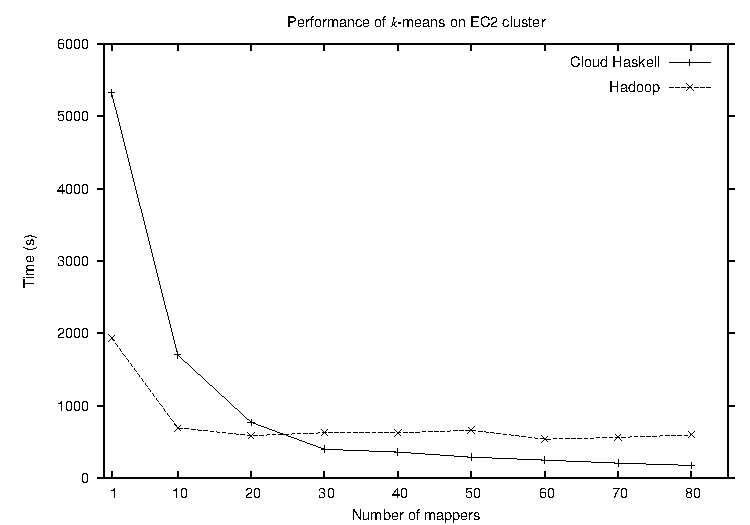
\includegraphics[width=\columnwidth]{ec2}
}
\caption{ 
\label{fig:performance1}
The run-time of the \kmeans{} algorithm in Cloud Haskell. The input data was one million 100-dimensional data points; we used one reducer nodes for all tests. % Performance improves at a better than linear rate as we increase the number of mapper nodes.
}
\end{figure}

The performance of \kmeans{} under Cloud Haskell does not compare favorably 
\apb{say how bad!} with systems such as Skywriting. Although the time needed to execute the algorithm reduces significantly as we add worker nodes, performance as an absolute is disappointing. We hope to partially remedy this situation with the improved process allocation to be introduced in our task layer, discussed in Section \ref{s:futureWork}.
\apb{Say we just got it running and have not optimized anything.}

% Isis/Paxos/virtual synchrony consensus?

\section{Related work} \label{s:related}

As should be clear, our main inspiration comes from Erlang, whose tremendous
success for distributed programming led us to emulate its best features.
A second inspiration is the Ciel execution engine and Skywriting language
of Murray \emph{et al} \cite{Murray2010, Murray2011}.

In scientific computing, the most scalable solution for distributed parallel computation is the Message Passing Interface (MPI). As its name suggests, MPI is similar to our framework in its preference for communication by messages. Unlike our framework, MPI is language-independent; interfaces are available for Fortran, C, and C++, and an array of different implementations have been optimized for a variety of supercomputer architectures.  In comparison, Cloud Haskell, as a DSL embedded in Haskell, is not easily available from other languages.
This is of course a weakness, but it is also a great strength.  
Haskell's type system separates shared-memory concurrency, distributed-memory concurrency and pure computation, giving programmers powerful reasoning tools that are not available when using a subroutine library called from a language with a weaker type system. 

There have been lots of mechanisms for executing functions on remote
systems, staring with Birrell and Nelson's RPC~\cite{birrel1984}.
Specific to Java is the Remote Method Invocation (RMI) mechanism
\cite{javarmi}. CORBA proides the Interface Description Language (IDL)
\cite{corbaidl} to define implementation-language-independent remote
functions. Web services often use the SOAP standard to implement
remote procedure call.  However, none of these mechanisms deal with the problem of transmitting first-class functions that capture their environment.
Although it may be argued that any object-oriented language that supports mobile objects does as a consequence also support mobile functions, there have been few full implementations of mobile objects.  A notable exception is Emerald~\cite{jul1988}, which dealt with the issue of environment capture  by copying the relevant parts of the environment into an object when it was created.  
All objects, including stack frames, were mobile; serialization was handled by the run-time system and depended on introspection.

Implementing a framework for distributed computing in Haskell has been
done before, in the form of Glasgow Distributed Haskell
\cite{gdh2001}. Unlike our work, it tries to maintain the semantics of
shared-memory concurrency in a distributed environment, rather than
insisting on message-based communication between nodes. We argue that this is 
undesirable because it gives the programmer no model for reasoning about the costs of the computation.  

Our operations on channels are somewhat reminiscent of Concurrent ML's events~\cite{reppy:book}.
However, Concurrent ML does not support distribution because that would be incompatible with its
model of synchronization.  paraML, an experimental variant of Concurrent ML, did have
a distributed implementation; its serialization mechanism was entirely built-in \cite{bailey:paraml}.

The Acute language does a very solid job of dealing with type-safe
marshalling, based on passing type representations at runtime
\cite{acute:jfp}.  Serialization is mostly built-in, with some
programmer control offered for ``rebinding'', when values should be
rebound rather than serialised.  HashCaml, currently in alpha-release, is a
variant of OCaml that supports type-safe distributed
programming, including serialization of function values.  Like Actue
it uses explicit type passing, the details of how the free variables
of function closures are marshalled are hazy.  Rossberg's language
Alice likewise supports type-safe distributed programming
\cite{rossberg:alice}.  
The Clean language supports type-safe saving of arbitrary values (including
function closures into files \cite{clean:dynamic-io}, and in a recent
paper proposes a mechanism for runtime solving of class constraints 
\cite[Sect 4.2]{clean:wgp10}.

All of these systems fundamentally regard serialization of closures
as a built-in service.  In contrast, our work puts the programmer in
complete control of serialization, via the usual type-class mechanism.
Exposing closure conversion is a significant burden --- albeit one that can be
relieved with some syntactic sugar --- but one allows the
programmer to reason about the cost of sending a message.
Similarly, explicit serialization will typically lose structure 
sharing within a transmitted value, whereas a built-in mechanism can retain it
--- but that is also true of any traversal of a data structure.
We do not argue that our approach is always better, but rather that it offers
a new and unexplored design point.

\section{Conclusions and Future Work}
%: \label{s:futureWork}
\label{s:futureWork}
Cloud Haskell, as presented in this paper, provides a good starting point for building a distributed application.  
However, as yet it is no more than this: we have a lot of work left to do to make ``Haskell in the Cloud'' a reality.

Our ongoing work is on two levels.
At the lower level, we plan to implement \textt{Static} and the corresponding type inference rules in GHC.  This will remove the need for the workarounds described in Section~\ref{s:faking}.
At the higher level, we have designed a framework that builds on the interface described here.
In it, the main unit of abstraction changes from the process to the \emph{task}: an idempotent, restartable block of code that produces a well-defined result. The task layer of the framework, like the process layer presented in this paper, is accessible as a domain-specific language (DSL) embedded in Haskell as a monad.

Whereas the DSL described here lets programmers start processes, exchange messages, and detect failure, the task-based framework takes care of allocating tasks to physical resources, resolving data dependencies between tasks, and automatically recovering from failure. 
To make this possible, the task layer represents the computation as a directed acyclic graph, in which tasks are the vertices and the data dependencies between then are the edges, and are exposed to the programmer as \emph{promises}.
We hope that the task layer will provide functionality similar to well-known distributed frameworks such as MapReduce~\cite{MapReduce2008} and Dryad~\cite{Dryad2007}, although our immediate inspiration comes from the Skywriting project~\cite{Murray2010,Murray2011}.

\acks
We particularly thank John Launchbury who helped us see that $\text{\tt Static}\;\tau$ for an arbitrary type $\tau$
would be an improvement over a static \emph{function} type 
$\sigma \nfn \tau$.  Andrew Black thanks Microsoft Research, Ltd, for providing a congenial home during his sabbatical.
Jeff Epstein would like to thank Alan Mycroft for his support and helpful feedback. 

% The bibliography should be embedded for final submission.

\bibliographystyle{abbrvnat}
\bibliography{bib}

%\bibliographystyle{abbrvnat}
%\begin{thebibliography}{}
%\softraggedright
%
%\bibitem[Smith et~al.(2009)Smith, Jones]{smith02}
%P. Q. Smith, and X. Y. Jones. ...reference text...
%
%\end{thebibliography}

\end{document}
